% Biografias ----------------------------------------------------------------
\section{Sobre os autores}

\begin{frame}{Quem está apresentando}
	\begin{columns}[c]
		\begin{column}{0.32\textwidth}
			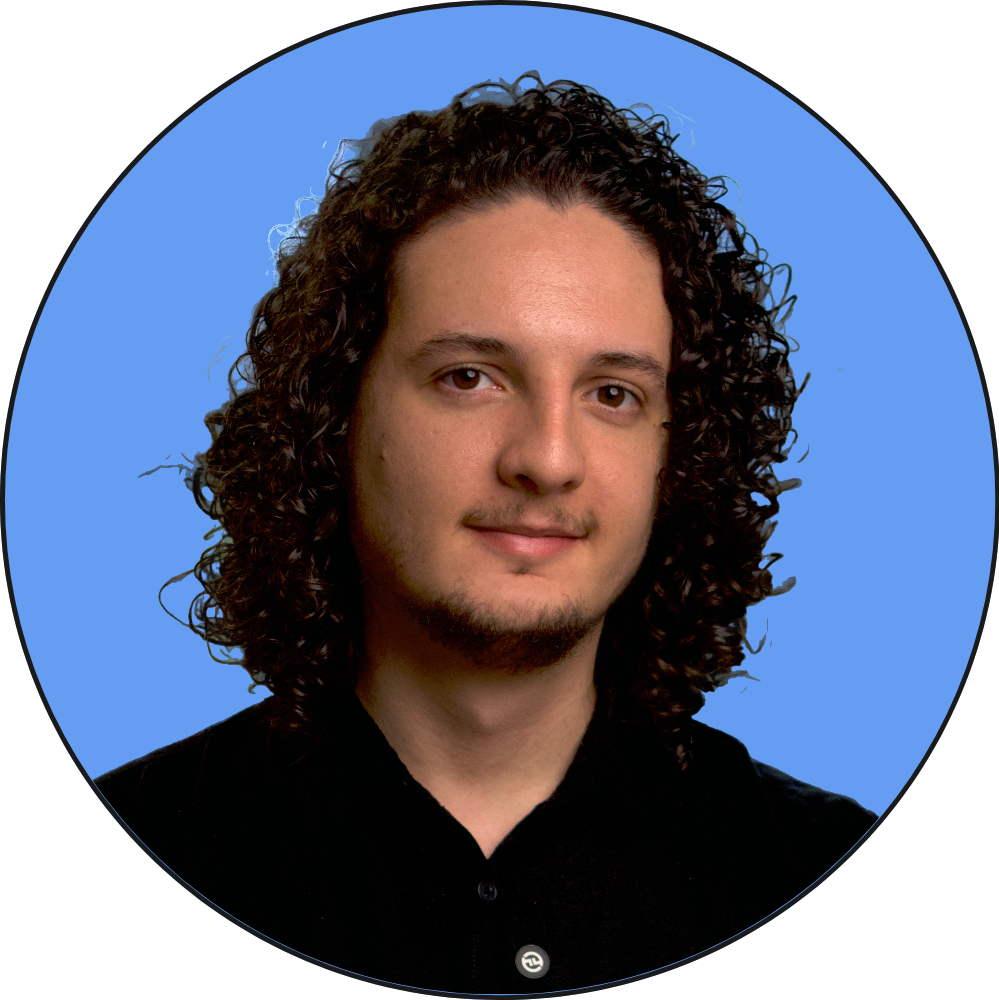
\includegraphics[width=\linewidth]{figures/gustavo_portait.png}
		\end{column}
		\begin{column}{0.66\textwidth}
			\textbf{Gustavo Ferreira Viegas de Oliveira (Apresentador)} \\
			{}
			[\href{https://lattes.cnpq.br/6788178534558304}{Lattes}]
			[\href{https://www.linkedin.com/in/gfviegas}{Linkedin}]

			\vspace{10pt}

			\small
			Bacharel e mestre em Ciência da Computação pela Universidade Federal de Viçosa (UFV). Minha dissertação
			desenvolveu o Causal-Nest (\cite{causal-nest-kbs}), framework que automatiza
			o pipeline de descoberta, estimação e refutação causal para profissionais
			de ML.
			\\ CTO e co-fundador da startup Hubs Contabilidade.
		\end{column}
	\end{columns}
\end{frame}

\begin{frame}{Orientadores}
	\textbf{Fabrício Aguiar Silva} [\href{http://lattes.cnpq.br/4039841663043863}{Lattes}]

	\small
	É doutor em Ciência da Computação pela UFMG (2015), com tese premiada
	como segunda melhor do Brasil pela SBC. Professor da UFV -- Campus Florestal
	desde 2010, atua em inteligência artificial aplicada e sistemas distribuídos.
	Orientador de mestrado do apresentador.

	\vfill
	\normalsize
	\textbf{Marcus Henrique Soares Mendes} [\href{https://lattes.cnpq.br/9729345585563115}{Lattes}]

	\small
	É doutor em Engenharia Elétrica pela UFMG (2013) e Professor Titular da
	UFV -- Campus Florestal desde 2005. Atua em otimização, computação evolutiva
	e meta-heurísticas. Co-orientador de mestrado do apresentador.
\end{frame}
